\documentclass[../../main.tex]{subfiles}
\begin{document}
\section{L'ordinateur}
\subsection{Vue de haut}
On peut considérer un ordinateur comme un système évoluant selon des entrées pour produire des sorties :
\begin{center}
  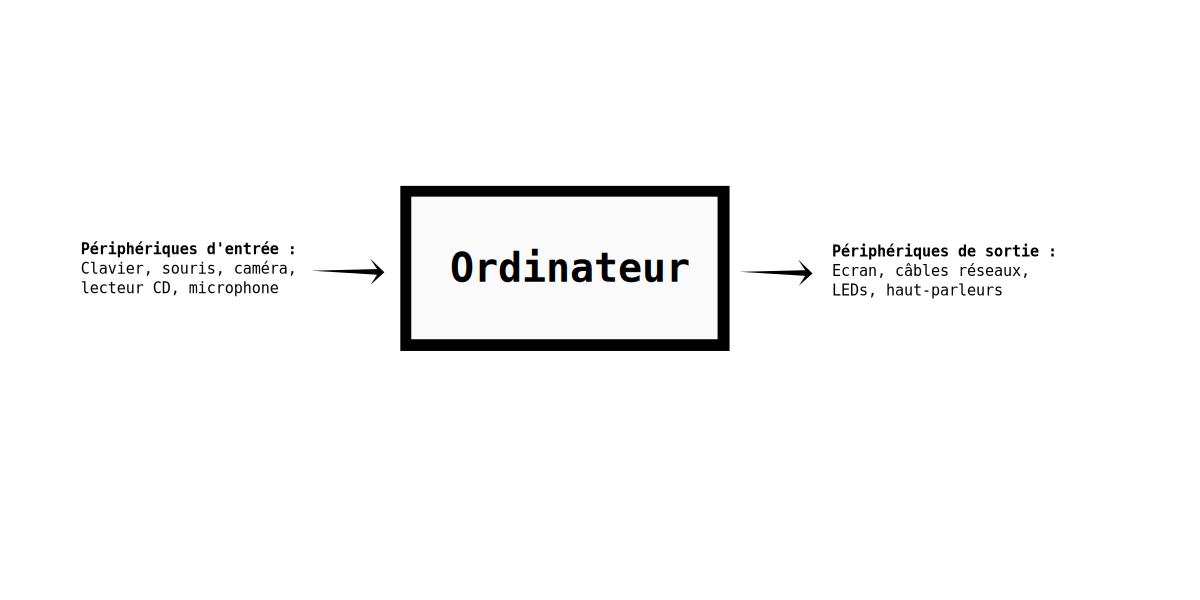
\includegraphics[width=\textwidth]{system}
\end{center}
Ces entrées et sorties sont captés et produites via des appareils appelés périphériques d'entrée/sortie. On garde généralement l'appellation en anglais \textit{\underline{I}nput/\underline{O}utput Drivers} ou simplement \textit{\underline{I}/\underline{O} Drivers}.

\begin{minitelbasicbox}{\textbf{Petit apparté :} De la rigueur de la définition d'un ``ordinateur''}
Un ordinateur est appareil qui ``calcule''. La signification mathématique du terme ``calculer'' n'a
rien d'évidente. Calculer est au départ une notion que l'on peut qualifier d'assez intuitive et il
est donc difficile d'apporter une définition formelle claire qui satisfasse ce qu'un humain peut
subjectivement appeler le ``calcul''.

La notion de calculabilité, qui définit ce qui est calculable et ce qui ne l'est pas, apporte une
définition du calcul. Cette notion est fondé sur des modèles fondamentaux du calcul (tous
équivalents, et heureusement !) comme les machines de Turing et le $\lambda$-calcul. Les ordinateurs
contemporains sont fondés sur le modèle de la machine de Turing et sont dits équivalents au
modèle de la machine de Turing.

Sans plus de détail\footnote{Pour plus de détail, voir le livre \cite{XFI}} car cela serait tout à fait hors-sujet, la machine de Turing est basiquement une bande infinie de caractères munit d'une tête de lecture/écriture qui se déplace latéralement
sur cette bande et agit selon la valeur des caractères lues grâce à une fonction de transition.
\end{minitelbasicbox}

Le symbole \textit{I/O} est extrêmement récurrent puisqu'il apparaît dans tous les cas où existe un système d'entrée et de sortie d'informations.
\subsection{À l'intérieur}
Les périphériques permettent l'interaction avec le système de l'ordinateur. Pourtant, celui-ci peut très bien fonctionner sans. Par exemple, on lisait les résultats des premiers ordinateurs directement à l'intérieur, et on y entrait les programmes ``à la main'', en modifiant les branchements des câbles pour ``écrire le programme''. En soi, cette notion d'écriture est assez récente, puisqu'elle date des ordinateurs disposant d'un clavier et d'un écran, périphériques d'entrée/sortie fondamentales pour une interaction ``facile'' avec un ordinateur.

L'ordinateur lui-même est uniquement un calculateur possédant une mémoire. Il est représenté de manière simplifié par le schéma suivant qui représente la modélisation d'un ordinateur appelée \textit{architecture de Von Neumann} :
\begin{center}
  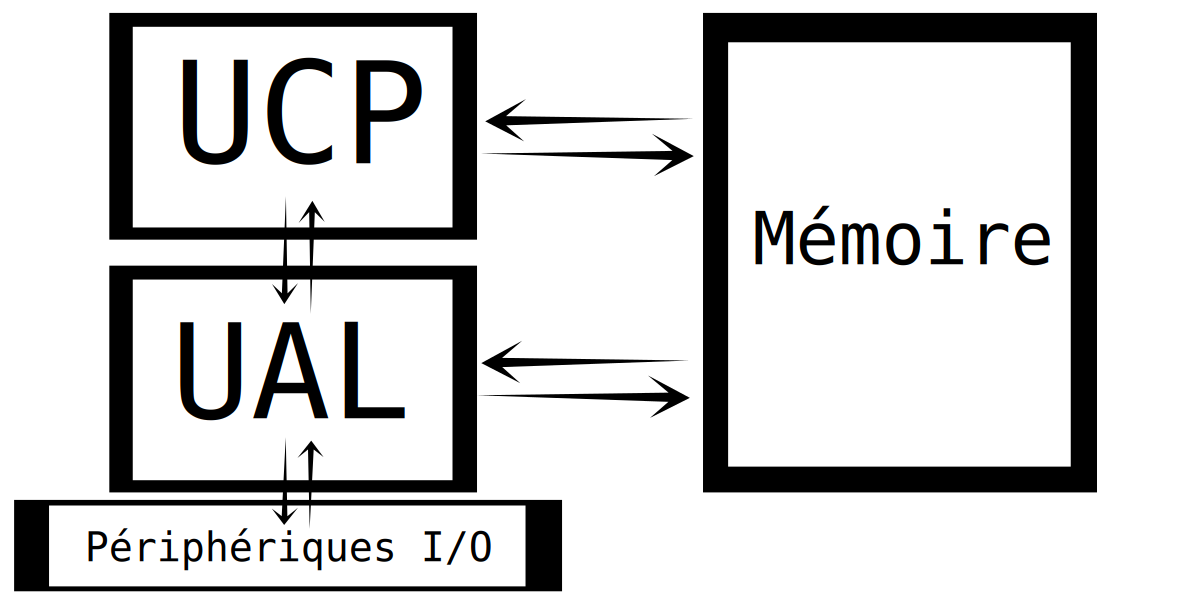
\includegraphics[height=6cm]{structure_von_neumann}
\end{center}
\textbf{UAL} signifie \underline{U}nité \underline{A}rithmétique et \underline{L}ogique. Ce système constitué de circuits informatiques permet d'effectuer toutes les opérations fondamentales de l'ordinateur, comme l'addition, la multiplication, la soustraction, la division, la lecture de la mémoire et l'écriture dans la mémoire.

\textbf{UCP} signifie \underline{U}nité de \underline{C}ontrôle de \underline{P}rogramme. Ce système supervise l'UAL, et contrôle son exécution. Il s'occupe en particulier de ``comprendre'' les instructions lues dans la mémoire pour faire exécuter par l'UAL les opérations correctes. Il effectue aussi le passage d'une instruction à l'autre.

Les registres forment un système de stockage de capacité très (très (très)) faible, destinés à stocker des valeurs temporaires. Ils servent en particulier de tampons pour les calculs de l'UAL et de l'UCP.

\textbf{Remarque 1 :} L'UCP et l'UAL, avec les registres, forment l'\textbf{UCC} (\underline{U}nité \underline{C}entrale de \underline{C}alcul, \textbf{CPU} en anglais).

\textbf{Remarque 2 :} Le schéma de l'ordinateur présenté ici permet de comprendre \textit{dans les grandes lignes} le fonctionnement d'un ordinateur, mais n'est ni complet ni particulièrement détaillé. Ainsi, ni l'alimentation, ni la carte mère, ni une potentielle carte graphique ne sont explicités ici. Ce schéma propose une vision très abstraite de ce qu'est un ordinateur et ne détaille rien des techniques mises en oeuvre.

La mémoire elle-même n'est dans les faits pas constituée d'un unique bloc mais de plusieurs supports de mémoire dont la vitesse et la capacité varient. On distingue par ordre de vitesse croissante et de capacité décroissante :
\begin{itemize}
    \item les bandes magnétiques (très lents, capacité native de $18\ To$ avec la technologie LTO-9, voir \url{https://fr.wikipedia.org/wiki/Linear_Tape-Open})
    \item les disques durs (lents, capacité allant de $250\ Go$ à $2\ To$)
    \item la mémoire RAM (pour \underline{R}andom \underline{A}ccess \underline{M}emory) (rapide, capacité allant de $1\ Go$ à $8\ Go$, et par agrégation jusqu'à $128\ Go$ voire plus).
    \item la mémoire SRAM  (pour \underline{S}tatic RAM) (5 à 10 fois plus rapide que la RAM, même capacité mais beaucoup plus chère)
    \item les registres (extrêmement rapide, capacité allant de 1 octet à 8 octets, 16 octets pour les ordinateurs spécialisés en calcul scientifique).
\end{itemize}
Ces types de support mémoire ne seront pas toutes détaillées dans la suite, en tout cas pas dans leur principe de fonctionnement. L'utilité de certains supports sera tout de même expliqué (notamment le disque dur et la mémoire RAM, ainsi que certains registres ultérieurement).

\textbf{Remarque :} En considérant seulement l'ensemble constitué de l'UAL et de l'UCP, la mémoire peut aussi être vue comme un support d'entrée/sortie. Ainsi, la lecture d''une information dans la mémoire constitue une entrée du système (UAL + UCP), et l'écriture d'une information dans la mémoire constitue une sortie du système (UAL + UCP).
\subsection{Données manipulées}
\subsubsection{Binaire}
Un ordinateur est une machine constituée de circuits électroniques. Les informations qui circulent à l'intérieur de celui-ci sont donc des signaux électriques, caractérisés par leur tension. Cette tension traduit deux états, pour des raisons de stabilité et de facilité d'implantation. Le premier état représente l'absence de tension ($U \approx 0\ V$), et le second état représente la présence d'une tension ($U \approx V_{ref} > 0$).

Le premier état est représenté par le chiffre\footnote{Il ne s'agit que d'un symbole sans signification.} 0 et le second par le chiffre\footnote{\textit{idem}} 1. Chaque chiffre (0 ou 1) est appelé un \textit{bit} (\textit{\underline{b}inary dig\underline{it}} en anglais). Cette modélisation sera justifiée par la suite de par les liens efficaces que l'on peut établir entre ces séquences d'états et $\mathbb{N}$.

Toutes les données manipulées par un ordinateur sont donc constituées de 0 et de 1. L'ensemble $\{0, 1\}$ est en théorie du langage un ensemble de \textit{lettres}. Une séquence de lettres est appelée un \textit{mot} et le langage binaire est l'ensemble des mots écrits avec l'alphabet $\{0, 1\}$. On ne peut pas encore appeler le mot $1000010$ un nombre puisqu'il ne lui est pour l'instant associé aucune interprétation numérique\footnote{Il existe des interprétations non numériques de mots binaires. Par exemple, on peut associer à chaque lettres \textit{a}, \textit{b}, \dots, \textit{z} un mot binaire spécifique. Cela revient à interpréter un mot binaire comme une lettre.}.
\subsubsection{Octets}
Pour structurer l'information, on regroupe ces bits par paquets de 8 appelés \textit{octets}. Un octet est donc un nombre écrit avec 8 bits.

On a ensuite les mêmes préfixes du système international que pour n'importe quelle unité physique :
\begin{itemize}
  \item $1\ Ko = 1000\ o$
  \item $1\ Mo = 1000\ Ko$
  \item $1\ Go = 1000\ Mo$
  \item $1\ To = 1000\ Go$
  \item $1\ Po = 1000\ To$
  \item etc\dots
\end{itemize}
Ainsi que d'autres préfixes plus spécifiques à l'informatique qui sont basés sur l'interprétation entière des mots binaires :
\begin{itemize}
  \item $1\ Kio \text{ (kibioctet)} = 2^{10}\ o = 1024\ o$
  \item $1\ Mio \text{ (mebioctet)} = 2^{10}\ Kio = 1024\ Kio$
  \item $1\ Gio \text{ (gibioctet)} = 2^{10}\ Mio = 1024\ Mio$
  \item $1\ Tio \text{ (tebioctet)} = 2^{10}\ Gio = 1024\ Gio$
  \item $1\ Pio \text{ (pebioctet)} = 2^{10}\ Tio = 1024\ Tio$
  \item etc\dots
\end{itemize}
\begin{minitelbasicbox}{\textbf{Petit apparté :} octet comme unité d'information}
L'octet est l'unité de l'information. Il permet de mesurer la quantitée d'information enregistrée (voir théorie de l'information de Shannon). En informatique pratique, il est utilisé comme mesure du stockage de l'information (ce qui est légèrement différent de la mesure de l'information qui est son sens premier). La pratique a donc légèrement déformé le sens originel du bit.

On parle d'ailleurs souvent d'un \textit{bit d'information}, qui fait référence à la théorie de l'information de Shannon.
\end{minitelbasicbox}
Les données sur un ordinateur sont mesurés en octets. La mémoire vive, ou d'un disque dur, consiste en un immense mot binaire, qui puisqu'il est divisé en groupes de 8 est en fait un immense tableau de cases de un octet chacune.

Le numéro de chaque case est appelé son adresse. La première case est d'adresse 0 et la dernière dans une mémoire de $T$ octets est $T-1$.
\section{Opérations logiques}
Les opérateurs sur les mots binaires sont des fonctions qui permettent d'agir sur les mots binaires, de les modifier.
\subsection{Arité d'un opérateur, d'une fonction}
Est appelé \textit{arité} d'une fonction son nombre de paramètres.

Un opérateur $1$-aire, dit \textit{unaire} (ou encore parfois \textit{monadique}), n'agit que sur une seule variable. Il ne possède qu'un seul paramètre.

Un opérateur $2$-aire, dit binaire, possède deux paramètres. Il agit sur deux variables. Par exemple, l'addition de deux nombres est une opération binaire.

Il est naturellement possible de considérer les opérations unaire sur un mot binaire de $N$ bits comme des fonctions $N$-aires, c'est-à-dire à $n$ paramètres. Par exemple, on pourrait considérer que l'inversion de bits d'un mot binaire de $N$ bits est en vérité une opération $N$-aire puisqu'elle agit sur $N$ bits qui constituent $N$ paramètres. De même, une opération binaire de deux mots de $N$ bits peut être considérée comme $2N$-aire.

Toutefois, après avoir posé $N$ comme le nombre de bits d'un mot binaire, un mot binaire de $N$ bits est \textit{par convention} considéré comme un unique paramètre pour l'ensemble des opérateurs. Ainsi, l'ensemble des opérateurs décrits ci-dessous sont des opérateurs unaires ou binaires uniquement.
\subsection{Opérations logiques et tables de vérité}
Les opérations dites \textit{logiques} sont des opérations qui s'effectuent sur les lettres de mots binaires sans nécessaire considération pour une quelconque interprétation numérique de ces mots.

Les \textit{tables de vérité} sont un moyen commode de visualiser les opérations logiques. Il s'agit de représenter toutes les sorties d'une fonction opératrice selon toutes les entrées possibles. Pour une fonction d'opérateur $N$-aire, on a $2^{N}$ possibilités d'entrées\footnote{En effet, il n'y a que deux lettres dans l'alphabet $\{0, 1\}$.}. Il faut décrire chacune des $2^{N}$ sorties associées pour décrire la fonction et ainsi l'opérateur.

\textbf{Remarque :} Il s'agit d'une définition de fonction dite \textit{par extension} dans laquelle on liste toutes les correspondances. La manière classique de décrire une fonction grâce à une expression\footnote{Comme $f\ :\ x\mapsto{x^{2}}$ par exemple} est appelée définition \textit{par compréhension}. Ce vocabulaire est emprunté à la théorie des ensembles puisqu'une fonction est un produit cartésien.

\textbf{Exemple :} Voici une table de vérité d'une fonction logique $f$ $3$-aire, dont on note les trois entrées $A$, $B$ et $C$ :
\begin{center}
\begin{tabular}{c|c|c|c}
$A$ & $B$ & $C$ & $f(A, B, C)$ \\
\hline
0 & 0 & 0 & 0 \\
0 & 0 & 1 & 0 \\
0 & 1 & 0 & 0 \\
0 & 1 & 1 & 1 \\
1 & 0 & 0 & 0 \\
1 & 0 & 1 & 1 \\
1 & 1 & 0 & 1 \\
1 & 1 & 1 & 1
\end{tabular}
\end{center}
On observe que le caractère \textit{exponentiel} du nombre d'entrées et de sorties rend cette représentation inutilisable pour des fonctions d'arité grande. \\
En interprétant la lettre/symbole 0 par le nombre 0 et la lettre/symbole 1 par le nombre 1, on peut aussi décrire $f$ par compréhension :
$$
\begin{array}{cclcl}
f & : & \{0, 1\}^{3} & \rightarrow & \{0, 1\} \\
  &   & (A, B, C) & \mapsto &  AB + BC + CA - 2ABC
\end{array}
$$
\subsection{Opérations logiques élémentaires}
Il existe quelques opérateurs logiques classiques très largement utilisés en informatique :
\begin{itemize}
	\item le OU logique exclusif
	\item le OU logique inclusif
	\item le ET logique
	\item le NON logique
\end{itemize}
On peut expliquer les noms donnés à ces opérateurs en considérant l'interprétation suivante des symboles 0 et 1 :
\begin{itemize}
	\item 0 correspond à la valeur logique \og Faux \fg{}
	\item 1 correspond à la valeur logique \og Vrai \fg{}
\end{itemize}
\subsubsection{OU logique inclusif}
L'opérateur binaire OU logique inclusif, noté $\vee$, est décrit par la table de vérité suivante :
\begin{center}
\begin{tabular}{c|c|c}
$A$ & $B$ & $A\vee{B}$ \\
\hline
0 & 0 & 0 \\
0 & 1 & 1 \\
1 & 0 & 1 \\
1 & 1 & 1 \\
\end{tabular}
\captionof{table}{Table de vérité de l'opérateur $\vee$}
\end{center}
$A\vee{B}$ est vraie si et seulement si l'une \textit{OU} l'autre des deux entrées est vraie.
\subsubsection{OU logique exclusif}
L'opérateur binaire OU logique exclusif, noté $\oplus$, est décrit par la table de vérité suivante :
\begin{center}
\begin{tabular}{c|c|c}
$A$ & $B$ & $A\oplus{B}$ \\
\hline
0 & 0 & 0 \\
0 & 1 & 1 \\
1 & 0 & 1 \\
1 & 1 & 0 \\
\end{tabular}
\captionof{table}{Table de vérité de l'opérateur $\oplus$}
\end{center}
$A\oplus{B}$ est vraie si et seulement si l'une \textit{OU} l'autre des deux entrées est vraie, mais pas les deux en même temps !
\subsubsection{ET logique}
L'opérateur binaire ET logique exclusif, noté $\wedge$, est décrit par la table de vérité suivante :
\begin{center}
\begin{tabular}{c|c|c}
$A$ & $B$ & $A\wedge{B}$ \\
\hline
0 & 0 & 0 \\
0 & 1 & 0 \\
1 & 0 & 0 \\
1 & 1 & 1 \\
\end{tabular}
\captionof{table}{Table de vérité de l'opérateur $\wedge$}
\end{center}
$A\wedge{B}$ est vraie si et seulement si les deux entrées sont vraies en même temps.
\subsubsection{NON logique}
Le NON logique $\neg$ est une fonction unaire/monadique :
\begin{center}
\begin{tabular}{c|c}
$A$ & $\neg{A}$ \\
\hline
0 & 1 \\
1 & 0 \\
\end{tabular}
\captionof{table}{Table de vérité de l'opérateur $\neg$}
\end{center}
Ainsi, $\neg{A}$ est vraie si et seulement si $A$ est faux et inversement.
\subsubsection{Extension aux mots}
On pose $\mathcal{B} = \{0, 1\}$ et $N\in{\mathbb{N}^{*}}$

Toutes les opérations décrites ci-dessus peuvent être étendues sur l'ensemble des $N$-uplets de $\mathcal{B}^{N}$. \newline
Soit $\ast\in{\{\vee, \wedge, \oplus\}}$. Soient $a, b \in{\mathcal{B}^{N}}, a = \begin{pmatrix}
a_0 \\
\vdots \\
a_{N-1}
\end{pmatrix}$ et $b = \begin{pmatrix}
b_0 \\
\vdots \\
b_{N-1}
\end{pmatrix}$. Alors :
$$a\ast{b} = \begin{pmatrix}
a_0 \ast{b_{0}}\\
\vdots \\
a_{N-1} \ast{b_{N-1}}
\end{pmatrix}$$
De plus (valable pour toute fonction logique monadique autre que $\neg$) :
$$\neg{v} = \begin{pmatrix}
\neg v_{0}\\
\vdots \\
\neg v_{N-1}
\end{pmatrix}$$
\subsection{Opérations de décalage}
\subsubsection{Décalage à gauche}
L'opérateur $\ll$ est défini comme suit :
$$
\begin{array}{lclcll}
\ll & : & \mathcal{B}^{N}\times{\llbracket0, N\rrbracket} & \rightarrow & \mathcal{B}^{N} \\
     &   & ((a_{N-1}\dots a_{0}), i) & \mapsto & a_{N-1-i}\dots a_{0}\underbrace{0\dots 0}_{\text{$i$ fois}} & \text{ si $i < N$} \\
     &   & & \mapsto & 0\dots 0 & \text{ si $i = N$}
\end{array}
$$
\subsubsection{Décalage logique à droite}
L'opérateur $\gg_{l}$ est défini comme suit :
$$
\begin{array}{lclcll}
\gg_{l} & : & \mathcal{B}^{N}\times{\llbracket0, N\rrbracket} & \rightarrow & \mathcal{B}^{N} \\
     &   & ((a_{N-1}\dots a_{0}), i) & \mapsto & \underbrace{0\dots 0}_{\text{$i$ fois}}a_{N-1}\dots a_{i} & \text{ si $i < N$} \\
     &   & & \mapsto & 0\dots 0 & \text{ si $i = N$}
\end{array}
$$
\subsection{Exercices}
Dans tous les exercices, $\mathcal{B} = \{0, 1\}$ et $N\in\mathbb{N}^{*}$

\exercise{La compréhension pour mieux comprendre} Décrire les fonctions $\vee$, $\oplus$, $\wedge$ et $\neg$ par compréhension.

\exercise{Universalité des fonctions logiques élémentaires} Montrer que toute fonction logique $N$-aire peut s'exprimer comme une combinaison des fonctions $\vee$, $\wedge$ et $\neg$.

\exercise{Porte NAND} On pose la fonction $\uparrow$ dite \og NAND \fg définie par :
$$
\begin{array}{lclcl}
\uparrow & : & \mathcal{B}^{2} & \rightarrow & \mathcal{B} \\
& & (A, B) & \mapsto & \neg{(A\wedge{B})}
\end{array}
$$
\begin{enumerate}
    \item Déterminer la table de vérité de l'opérateur NAND
    \item Exprimer chacune des fonctions $\vee$, $\wedge$ et $\neg$ par compréhension en utilisant uniquement la fonction $\uparrow$
\end{enumerate}
\textit{\underline{Note :} Un opérateur capable d'exprimer les opérateurs logiques élémentaires à lui seul est dit \og universel \fg}

\exercise{Porte NOR} On pose la fonction $\downarrow$ dite \og NOR \fg définie par :
$$
\begin{array}{lclcl}
\downarrow & : & \mathcal{B}^{2} & \rightarrow & \mathcal{B} \\
& & (A, B) & \mapsto & \neg{(A\vee{B})}
\end{array}
$$
\begin{enumerate}
    \item Déterminer la table de vérité de l'opérateur NOR
    \item Montrer que $\downarrow$ est un opérateur universel.
\end{enumerate}
\exercise{Petit retour à l'algèbre fondamentale} Démontrer que $G = (\mathcal{B}^{N}, \oplus)$ est un groupe commutatif. Pour tout $b\in{\mathcal{B}^{N}}$, déterminer $b^{-1}$.
\\
\textit{\underline{Rappel :} Un groupe est un ensemble $E$ muni d'une loi de composition interne $\ast$ associative respectant les propriétés suivantes :
\begin{enumerate}
    \item il existe un unique élément neutre $e$ tel que pour tout $x\in{E}$, $x\ast{e} = e\ast{x} = x$
    \item chaque élément $x\in{E}$ admet un inverse $x^{-1}$, c'est-à-dire tel que $x\ast{x^{-1}} = x^{-1}\ast{x} = e$.
\end{enumerate}
Un groupe est commutatif si $\ast$ est commutative.}

\exercise{Inversibilité des décalages} Est-ce que les décalages logiques droit et gauche sont inversibles ? Justifier.
\section{Opérations arithmétiques}
Sont ici décrites les opérations arithmétiques sur $\mathcal{B}^{N}$. L'arithmétique définit est une arithmétique modulaire, c'est-à-dire que l'ensemble $\llbracket 0; 2^{N}\llbracket$ est assimilé à l'ensemble des représentants des classes d'équivalence de $\dfrac{\mathbb{Z}}{2^{N}\mathbb{Z}}$.
\subsection{Représentation d'un nombre entier en binaire}
On considère la fonction suivante :
$$
\begin{array}{lclcl}
btoi_{u} & : & \mathcal{B}^{N} & \rightarrow & \llbracket 0; 2^{N}\llbracket \\
     &   & b & \mapsto & \displaystyle\sum_{i = 0}^{N-1}(b_{i}2^{i})
\end{array}
$$
Cette fonction calcule la valeur numérique d'un mot binaire. Il s'agit de l'interprétation d'un $N$-uplet de bits comme écriture en base 2 d'un nombre entier naturel (sans signe : \textit{\underline{u}nsigned} en anglais). Comme l'écriture d'un nombre en base 2 existe et est unique pour tout nombre naturel, il s'agit d'une bijection de $\mathcal{B}^{N}$ dans $\llbracket 0; 2^{N}\llbracket $. \newline
Sous la forme d'un polynôme de Horner évalué en 2 on a :
\begin{equation}\label{horner}
btoi_{u}(b) = b_{0} + 2(b_{1} + 2(b_{2} + 2(\dots)\dots))
\end{equation}
On écrit plus simplement :
$$n = (b_{N-1}b_{N-2}\dots b_{1}b_{0})_{2} = btoi_{u}(b)$$
Cette écriture est appelée représentation en base 2 de $n$, ou encore représentation binaire de $n$.

\textbf{Remarque :} On peut trouver la représentation en base 2 de $n$ par des divisions entières successives par 2 grâce à l'équation (\ref{horner}). Pour tout $i\in{\llbracket{0; N-1}\rrbracket}$, on a $b_{i} \equiv{\left\lfloor{\dfrac{n}{2^{i}}}\right\rfloor{[2]}}$ 

Cette remarque vient également corroborer l'expression de $btoi^{-1}$ :
$$
\begin{array}{lclcl}
btoi^{-1} & : & \mathbb{Z} & \rightarrow & \mathcal{B}^{N} \\
     &   & n & \mapsto & \begin{pmatrix}
n\ \%\ 2 \\
\vdots \\
\left\lfloor\dfrac{n}{2^{i}}\right\rfloor\ \%\ 2 \\
\vdots \\
\left\lfloor\dfrac{n}{2^{N-1}}\right\rfloor\ \%\ 2
\end{pmatrix}
\end{array}
$$
où l'opération \textit{modulo} noté $\%$ est définit pour tout $a, b\in{\mathbb{Z}}$ par $a\ \%\ b = a - b\left\lfloor\dfrac{a}{b}\right\rfloor$, c'est-à-dire qu'en posant la division euclidienne de $a$ par $b$, il existe un unique $q$ tel que $a = bq + (a\ \%\ b)$ et $0 \leq a\ \%\ b < b$

Par exemple, trouvons la représentation binaire de $53$ :
\begin{itemize}
     \item $\left\lfloor{\dfrac{53}{2^{0}}}\right\rfloor = 53 \equiv{1}[2]$
     \item $\left\lfloor{\dfrac{53}{2^{1}}}\right\rfloor = 26 \equiv{0}[2]$
     \item $\left\lfloor{\dfrac{26}{2^{2}}}\right\rfloor = 13 \equiv{1}[2]$
     \item $\left\lfloor{\dfrac{13}{2^{3}}}\right\rfloor = 6 \equiv{0}[2]$
     \item $\left\lfloor{\dfrac{6}{2^{4}}}\right\rfloor = 3 \equiv{1}[2]$
     \item $\left\lfloor{\dfrac{3}{2^{5}}}\right\rfloor = 1 \equiv{1}[2]$
     \item On s'arrête car $2^{6} > 53$. Du fait de la partie entière, toutes les prochaines divisions donneront 0.
\end{itemize}
D'où $53 = 1\times{2^{5}} + 1\times{2^{4}} + 0\times{2^{3}} + 1\times{2^{2}} + 0\times{2^{1}} + 1\times 2^{0} = (110101)_{2}$

\exercise{Conversion en binaire}\newline
Trouver la représentation binaire des dix entiers naturels ci-dessous :

\begin{minipage}{0.5\textwidth}
\begin{itemize}
     \item $76$
     \item $188$
     \item $33$
     \item $109$
     \item $92$
\end{itemize}
\end{minipage}
\begin{minipage}{0.5\textwidth}
\begin{itemize}
     \item $211$
     \item $4$
     \item $238$
     \item $161$
     \item $126$
\end{itemize}
\end{minipage}

Ici sont détaillées l'ensemble des opérations logiques et arithmétiques les plus communes qui peuvent être appliquées aux $N$-uplets de $B^{N}$. La bijection $btoi$ sera considéré implicitement pour la suite, c'est-à-dire que toute fonction ou relation appliquable sur $\mathcal{B}^{N}$ le sera aussi sur $\llbracket 0; 2^{N}\llbracket $, en considérant un nombre par sa représentation binaire.

Plus formellement, pour toute fonction $\ast : \mathcal{B}^{N} \rightarrow E$, on peut considérer de manière équivalente la fonction :
$$
\begin{array}{lclcl}
\ast_{\mathbb{N}} & : & \llbracket 0;2^{N}\llbracket  & \rightarrow & E \\
     &   & n & \mapsto & \ast{(btoi^{-1}{(n)})}
\end{array}
$$
\subsection{Nombres signés}
Pour représenter des nombres \textit{signés}, c'est-à-dire dont la valeur peut être négative comme positive (nombres qui possèdent un signe), on considère comme représentants de $\dfrac{\mathbb{Z}}{2^{N}\mathbb{Z}}$ les nombres : $\dot{(-2^{N-1})}, \dots, \dot{-1}, \dot{0}, \dot{1}, \dots, \dot{(2^{N-1}-1)}$

Soit $v\in{\mathcal{B}^{N}}$ quelconque.
$$
\begin{array}{lclcl}
btoi_{s} & : & \mathcal{B}^{N} & \rightarrow & \llbracket 2^{N-1}; 2^{N-1}\llbracket  \\
     &   & b & \mapsto & \displaystyle\sum_{i = 0}^{N-2}(b_{i}2^{i}) - b_{N-1}2^{N-1}
\end{array}
$$
\textbf{Remarque :} Si $b_{N-1} = 0$, alors $btoi_{u}(v) = btoi_{s}(v)$.

\proposition{} $\dot{(btoi_{s}(v))} = \dot{(btoi_{u}(w))} \Leftrightarrow v = w$

\textbf{Démonstration :} $(btoi_{s}(v)) \equiv \displaystyle\sum_{i = 0}^{N-2}(b_{i}2^{i}) - b_{N-1}2^{N-1} + b_{N-1}2^{N} [2^{N}]$ \newline
Donc $\dot{(btoi_{s}(v))} = \dot{(btoi_{u}(v))}$, or la représentation en base 2 d'un entier naturel est unique, donc $v = w$.

\textbf{Interprétation :} Quelque soit l'interprétation du mot binaire (signé ou non signé), la représentation binaire est unique. Ainsi, la proposition précédente est équivalente à $\forall{x, y\in{\mathbb{Z}}}, \dot{x} = \dot{y} \Leftrightarrow btoi^{-1}(x) = btoi^{-1}(y)$

\proposition{} $b_{N-1} = 1 \Leftrightarrow btoi_{s}(v) < 0$.

\textbf{Démonstration :} $\displaystyle\sum_{i = 0}^{N-2}(b_{i}2^{i})$ est majoré par $\displaystyle\sum_{i = 0}^{N-2}(2^{i}) = 2^{N-1} - 1 < b_{N-1}2^{N-1}$

\textbf{Interprétation :} Il suffit de regarder le bit de poids fort d'un nombre pour connaître son signe.

\proposition{} $btoi_{s}(v) = -(btoi_{s}(\neg{v}) + 1)$

\textbf{Démonstration :}
\[
\begin{array}{lcl}
-(btoi_{s}(\neg{v}) + 1) & = & -(\displaystyle\sum_{i = 0}^{N-2}((1-b_{i})2^{i}) - (1-b_{N-1})2^{N-1} + 1) \\
& = & \displaystyle\sum_{i = 0}^{N-2}((b_{i}2^{i}) - \displaystyle\sum_{i = 0}^{N-2}(2^{i}) + (1 - b_{N-1})2^{N-1} - 1 \\
& = & \displaystyle\sum_{i = 0}^{N-1}((b_{i}2^{i}) - 2^{N-1} - b_{N-1}2^{N-1} \\
& = & btoi_{s}(v)
\end{array}
\]
\subsection{Addition}
On définit l'opération d'addition de deux $N$-uplets de $\mathcal{B}^{N}$ comme l'opération :
$$
\begin{array}{lclcl}
+ & : & \mathcal{B}^{N}\times{\mathcal{B}^{N}} & \rightarrow & \mathcal{B}^{N} \\
  &   & (x, y) & \mapsto & btoi^{-1}(btoi_{u}(x) + btoi_{u}(y)) \\
\end{array}
$$
\textbf{Interprétation :} Il s'agit en fait de l'addition des deux nombres en base 2 (comme on additionne des nombres en base 10, ou $b$) dont on ne garde que les $N$ premiers bits. Ainsi, si on effectue l'addition $2^{N-1} + 2^{N-1}\notin{\llbracket 0; 2^{N}\llbracket}$, il faudrait un bit supplémentaire pour stocker l'information. Or ce bit n'est pas présent, il est donc simplement ignoré.

\proposition{Pseudo-linéarité} $\forall{x, y\in{\llbracket 0; 2^{N}\llbracket}}, x + y \equiv btoi_{u}(btoi^{-1}(x) + btoi^{-1}(y)) [2^{N}]$

\textbf{Démonstration :}

\[
\begin{array}{lcl}
\dot{btoi_{u}(btoi^{-1}(x) + btoi^{-1}(y))} & = & \dot{btoi_{u}(btoi^{-1}(btoi_{u}(btoi^{-1}(x))) + btoi_{u}(btoi^{-1}(y)))} \\
 & = & \dot{(btoi_{u}(btoi^{-1}(x)) + btoi_{u}(btoi^{-1}(y)))} \\
 & = & \dot{(btoi_{u}(btoi^{-1}(x)))} + \dot{(btoi_{u}(btoi^{-1}(y)))} \\
 & = & \dot{x} + \dot{y} \\
 & = & \dot{(x + y)}
\end{array}
\]
\textbf{Interprétation :} Additionner deux entiers naturels directement ou d'abord représenter en binaire ces entiers et ensuite additionner produit le même résultat modulo $2^{N}$ par la représentation sur $N$ bits.

\textbf{Exemples : (pour $N = 8$)}
\begin{itemize}
  \item $(0011\ 0101)_{2} + (0001\ 1000)_{2} = (0100\ 1101)_{2}$\newline
    c'est-à-dire $53 + 24 = 77$
  \item $(1000\ 1000)_{2} + (0000\ 1111)_{2} = (1001\ 0111)_{2}$\newline
    c'est-à-dire $136 + 15 = 151$ en non signé et $-120 + 15 = -105$ en signé
  \item $-(0101\ 1100)_{2} = (1010\ 0100)_{2}$\newline
    c'est-à-dire $-92 = 164$ en non signé et $-92 = -92$ en signé
  \item $(0111\ 1100)_{2} + (0100\ 1001)_{2} = (1100\ 0101)_{2}$\newline
    c'est-à-dire $124 + 73 = 197$ en non signé et $124 + 73 = -59$ en signé
  \item $(1110\ 1110)_{2} + (0010\ 1111)_{2} = (1001\ 1101)_{2}$\newline
    c'est-à-dire $238 + 47 = 29$ en non signé et $-18 + 47 = 29$ en signé
\end{itemize}
\subsection{Soustraction}
En utilisant la \textbf{Propriété 3.}, on définit simplement l'opération de soustraction par :
$$
\begin{array}{lclcl}
- & : & \mathcal{B}^{N}\times{\mathcal{B}^{N}} & \rightarrow & \mathcal{B}^{N} \\
     &   & (x, y) & \mapsto & x + (-y) = x + (\neg{y} + 1)
\end{array}
$$
\subsection{Décalage arithmétique à droite}
Au contraire du décalage logique à droite qui ne prend en considération aucune interprétation d'un mot binaire, le décalage arithmétique prend en considération le signe du nombre représenté par le mot binaire.

L'opération $\gg_{a}$ est définit comme suit :
$$
\begin{array}{lclcll}
\gg_{a} & : & \mathcal{B}^{N}\times{\llbracket0, N\rrbracket} & \rightarrow & \mathcal{B}^{N} \\
     &   & ((a_{N-1}\dots a_{0}), i) & \mapsto & \underbrace{a_{N-1}\dots a_{N-1}}_{\text{$i$ fois}}a_{N-1}\dots a_{i} & \text{ si $i < N$} \\
     &   & & \mapsto & a_{N-1}\dots a_{N-1} & \text{ si $i = N$}
\end{array}
$$
$\gg_{a}$ conserve le signe, puisque le bit de poids fort reste constant (voir \textbf{Propriété 2.}).

\proposition{} $\forall{v\in{\mathcal{B}^{N}}}, btoi_{u}(v\gg_{l}1) = \left\lfloor\dfrac{btoi_{u}(v)}{2}\right\rfloor$

\textbf{Démonstration :} Soit $v = v_{N-1}\dots v_{0}\in{\mathcal{B}^{N}}$.
\[
\begin{array}{lcll}
btoi_{u}(v\gg_{l}1)  & = & btoi_{u}(0v_{N-1}\dots v_{1}) \\
& = & \displaystyle\sum_{i = 1}^{N-1}(v_{i}2^{i-1}) + \underbrace{\left\lfloor\dfrac{v_{0}}{2}\right\rfloor}_{=0} \\
& = &  \left\lfloor\dfrac{btoi_{u}(v)}{2}\right\rfloor & \text{ car $\forall{(n, x)}\in{\mathbb{N}\times{\mathbb{R}}}, n + \lfloor{x}\rfloor = \lfloor{n + x}\rfloor$}
\end{array}
\]
\proposition{} $\forall{v\in{\mathcal{B}^{N}}}, btoi_{s}(v\gg_{a}1) = \left\lfloor\dfrac{btoi_{s}(v)}{2}\right\rfloor$

\textbf{Démonstration :} Soit $v = v_{N-1}\dots v_{0}\in{\mathcal{B}^{N}}$.
\[
\begin{array}{lcl}
btoi_{s}(v\gg_{a}1)  & = & btoi_{s}(v_{N-1}v_{N-1}\dots v_{1}) \\
& = & \displaystyle\sum_{i = 1}^{N-1}(v_{i}2^{i-1}) - v_{N-1}2^{N-1} + \underbrace{\left\lfloor\dfrac{v_{0}}{2}\right\rfloor}_{=0} \\
& = &  \left\lfloor{\displaystyle\sum_{i = 0}^{N-1}(v_{i}2^{i-1}) - v_{N-1}2^{N-1}}\right\rfloor \\
& = &  \left\lfloor{\displaystyle\sum_{i = 0}^{N-2}(v_{i}2^{i-1}) - v_{N-1}2^{N-2}}\right\rfloor \\
& = & \left\lfloor\dfrac{btoi_{s}(v)}{2}\right\rfloor
\end{array}
\]
\textbf{Remarque :} $btoi_{s}(v\gg_{a}1) = \left\lfloor\dfrac{btoi_{u}(v)}{2}\right\rfloor$ et $btoi_{u}(v\gg_{a}1) = \left\lfloor\dfrac{btoi_{s}(v)}{2}\right\rfloor$ ne sont vraies \textit{a priori} que pour des entiers naturels. En effet, le bit de signe ne doit pas être conservé en représentation non signée alors qu'il doit l'être en représentation signée.
\section{Opérations flottantes}
Les résultats qui vont suivre sont beaucoup plus spécifique à une partie mineure de l'informatique. Par manque de temps pour la rédaction, ils n'ont pas pu être particulièrement développés. Cela sera fait dans une version future. Veuillez excuser d'avance pour le manque de rigueur et de détails\dots\footnote{On rate en particulier le lien extraordinaire entre interprétation entière et interprétation flottante par la norme \textit{IEEE 754} des mots binaires qui fournie une approximation du logarithme, justifie ainsi le maintien de la relation d'ordre par changement d'interprétation et donc également la raison d'être de cette norme.}
\subsection{Représentation des nombres à virgules}
La manipulation de valeurs réelles est extrêmement importante, et même nécessaire, pour la manipulation d'espaces continues. On peut en particulier penser à des simulations physiques.

Pourtant, on peut observer simplement qu'un ordinateur manipule des données finies. En ce sens, il n'est envisageable de ne manipuler que des sous-ensembles de $\mathbb{Q}$. Par exemple :
\begin{itemize}
     \item $\pi$ possède un nombre infini de chiffres dont l'information ne peut être stockée par une formule \textit{calculable}\footnote{En informatique, une fonction est dite \textit{calculable} si il existe un algorithme qui pour tout $x$, détermine $f(x)$ en temps fini.}
     \item $\dfrac{1}{3}$ possède un nombre infini de chiffres après la virgule. Il suffit de stocker la partie entière $0$ ainsi que la partie répétée des décimales, c'est-à-dire $3$ (avec l'information de la répétition)
     \item $1.414$ possède un nombre fini de chiffres après la virgule. Il suffit alors de stocker deux entiers : celui avant la virgule, et celui après.
\end{itemize}
Dépendamment du type de nombre manipulé (avec un nombre infini de chiffre après la virgule ou non), le stockage des informations contenus par ce nombre diffère (et est parfois impossible comme dans le cas de $\pi$).

\textbf{Remarque 1 :} pour qu'un programme informatique manipulant des nombres à virgules puisse être exécuté sur plusieurs machines différentes, il faut que toutes ces machines aient la même représentation des nombres à virgules. Une norme est donc nécessaire.

\textbf{Remarque 2 :} Les processeurs d'ordinateur classiques\footnote{Comme les processeurs \textit{Intel x86}} manipulent des mots binaires de taille fixe $N\in\{8, 16, 32, 64, 80, 128\}$

\textbf{Remarque 3 :} Un mot de taille $N = 16$ ne peut représenter que quelques milliers de valeurs différentes ($2^{16} = 65536$) ce qui est ridicule pour représenter dans la pratique des nombres à virgules un tant soit peu différents.

\textbf{Remarque 4 :} Imaginons qu'on choisisse de représenter \textit{naïvement} des nombres à virgules sur $N = 32$ bits en stockant sur 16 bits la partie entière et la partie flottante. Cela limite particulièrement la précision des nombres représentés puisqu'il ne peut y avoir que $65536$ parties fractionnaires différentes.

Une norme est donc née de l'\textit{\underline{I}nstitute of \underline{E}lectrical and \underline{E}lectronics \underline{E}ngineers} (\textit{IEEE}), nommée la norme \textit{IEEE 754}. Il s'agit de la norme la plus largement utilisé en informatique, qui se base sur la notation scientifique.
\subsection{Écriture en base 2 de nombres décimaux}
Avant de décrire la norme \textit{IEEE 754}, on commence par détailler l'écriture en base 2 d'un nombre réel. 
On rappel qu'un nombre $x\in{\mathbb{R}}$ s'écrit de manière générique en base 10 sous la forme suivante :
$$x = \lfloor{x}\rfloor + fract(x)$$
La partie entière de $x$ s'écrit en base 10 : 
$$\lfloor{x}\rfloor = c_{n-1}10^{n-1} + c_{n-2}10^{n-2} + \dots + c_{0}10^{0}\text{, où $n = \lceil log_{10}(\lfloor{x}\rfloor)\rceil$}$$
Tandis que la partie fractionnaire de $x$ s'écrit en base 10 :
$$fract(x) = c_{-1}10^{-1} + c_{-2}10^{-2} + \dots$$
avec pour tout $i\in\mathbb{Z}$, $c_{i}\in{\llbracket{0; 9\rrbracket}}$

En changeant de base, et en choisissant la base 2, on a de manière équivalente :
$$\left\{\begin{array}{lcll}
\lfloor{x}\rfloor & = & c_{n-1}2^{n-1} + c_{n-2}2^{n-2} + \dots + c_{0}2^{0} & \text{, où $n = \lceil log_{2}(\lfloor{x}\rfloor)\rceil$} \\
fract(x) & = & c_{-1}2^{-1} + c_{-2}2^{-2} + \dots
\end{array}\right.$$
avec pour tout $i\in\mathbb{Z}$, $c_{i}\in{\llbracket{0; 1\rrbracket}}$

On relève au passage la propriété qui permet de calculer la représentation en base $b$ d'un nombre réel $x$ :

\proposition{} $\forall{n\in{\mathbb{N}^{*}}}, \lfloor b^{n}fract(x)\rfloor \equiv c_{(-n)}[b]$, où $c_{(-i)}$ est le $i^e$ après la virgule dans l'écriture de $x$ en base $b$.

\textbf{Exemple :} On peut appliquer récursivement cette propriété sur $x = 21.125 = (10101)_{2} + 0.125$ :
\begin{itemize}
     \item $c_{-1} = \lfloor 2^{1}\times{0.125} \rfloor = \lfloor 0.25\rfloor = 0$
     \item $c_{-2} = \lfloor 2^{2}\times{0.125} \rfloor = \lfloor 0.5\rfloor = 0$
     \item $c_{-3} = \lfloor 2^{3}\times{0.125} \rfloor = \lfloor 1\rfloor = 1$
     \item $\forall{i < -3}, c_{(-i)} = 0$
\end{itemize}
d'où : $x = (10101.001)_{2}$

On peut ainsi calculer la notation scientifique en base $b = 2$ de tout réel $x$ (voir section suivante)

\exercise{Écriture en base 2 de nombres non entiers} Écrire en base 2 les nombres suivants :
\begin{itemize}
     \item $14.5625$
     \item $1.40625$
     \item $7.4375$
     \item $0.1$ : Que remarque-t-on ? Exhiber un exemple d'un tel phénomène en écriture décimale.
\end{itemize} 
\subsection{Norme \textit{IEEE 754}}
Ne seront décrits ici que les nombres à virgules suivant la norme \textit{IEEE 754} d'une taille $N = 32$. En effet, le principe est le même pour les autres tailles si ce n'est que certaines constantes diffèrent.

\textbf{Rappel de vocabulaire en notation scientifique :} Un nombre $x\in{\mathbb{R}}$ en notation scientifique est écrit selon le format suivant :
$$x = \pm\ mantisse \times{base^{exposant}}$$
avec $mantisse\in{[1, base[}$ et $exposant\in{\mathbb{Z}}$

Par exemple :
$$+ 5.56\times{7^{-12}}$$
Ici :
\begin{itemize}
     \item $+$ est le \textit{signe} du nombre
     \item $5.56$ est la \textit{mantisse} du nombre
     \item $-12$ est l'\textit{exposant} du nombre
     \item $7$ est la \textit{base de représentation} du nombre
\end{itemize}
Dans toute la suite, la base de représentation sera fixe et vaudra $2$. Il n'y aura donc pas besoin de la stocker explicitement dans le mot binaire.

Il reste donc trois éléments, qui seront chacun stockés sur un certain nombre de bits. \newline
Selon la norme \textit{IEEE 754}, sur 32 bits :
\begin{itemize}
     \item le signe $s$ : 1 bit
     \item la mantisse $m$ : 23 bits
     \item l'exposant $e$ : 8 bits
\end{itemize}
Visuellement :
$$\underbrace{0}_{s}\underbrace{00000000}_{e}\underbrace{00000000000000000000000}_{m}$$
\textbf{Calcul du signe :} si $x < 0$, $s = 1$, et $s= 0$ sinon.

\textbf{Calcul de la mantisse :} Soit $x\in{\mathbb{R}}$.\newline
En base 2, il existe $(c_{i})_{i\in{\mathbb{Z}}}\in{\{0, 1\}^{\mathbb{Z}}}$ une suite unique telle que $x = \pm \displaystyle\sum_{i = -\infty}^{N}\left(c_{i}2^{i}\right)$ où $N$ est minimal.\newline
On a :
$$x = \pm 2^{N}\displaystyle\sum_{i = -\infty}^{N}\left(c_{i}2^{i-N}\right) = \pm m\times{2^{N}}\text{où $1 \leq m < 2$}$$
Il s'agit très exactement de l'écriture de $x$ en notation scientifique en base 2 et on peut calculer les $c_{i}$ grâce à l'algorithme déductible de la propriété de la section précédente.

Par ailleurs, on sait que $m\geq{1}$, il n'y a donc pas besoin de stocker cette information. On ne conserve pour la mantisse dans la représentation en norme \textit{IEEE 754} que les bits après la virgule.

\textbf{Calcul de l'exposant :} L'exposant peut être positif ou négatif. Cependant, on utilise pas ici la technique du complément à deux. En effet, cela rendrait plus complexe la comparaison entre deux nombres à virgules représentés selon cette norme.\footnote{La démonstration ne sera pas donnée mais la relation d'ordre sur les nombres réels représentés par les mots binaires est la même que celle sur les mots binaires réprésentant les nombres réels. C'est-à-dire qu'on peut indifférement comparer représentants ou représentés.} À la place, on utilise un \textit{biais}.

Si l'exposant est écrit sur $n$ bits, la valeur du biais est $2^{n-1} - 1$. Cette valeur est donc constante une fois la norme fixé (puisqu'on fixe le nombre de bits sur lesquels sera écrit l'exposant). On ajoute ce biais à la valeur $N$ trouvé lors du calcul de la mantisse. Ainsi, pour $N\in{\llbracket -2^{n-1} - 1; 2^{n-1}-1\rrbracket}$, on a $N + biais \geq{0}$ et donc représentable par un mot binaire interprété comme non signé.

\textbf{Remarque :} On interdit $N = 2^{n-1}$ (pour pouvoir représenter les valeurs spéciales $\pm\infty$ et $NaN$)

\textbf{Représentation finale :}

On distingue alors deux catégories selon la valeur de $N + biais$ pour le choix de la mantisse :
\begin{itemize}
     \item $N + biais = 0$ : le nombre est dit \textit{``dénormalisé''}
     \item $N + biais \in{\llbracket{1; 2^{n}-2\rrbracket}}$ : le nombre est dit \textit{``normalisé''}
\end{itemize}
La normalisation du nombre affecte en partie la valeur de la mantisse et de l'exposant encodé :

\textbf{Nombre normalisé :} on garde pour la mantisse les chiffres $c_{N-1}\dots c_{N-23}$.

\textbf{Nombre dénormalisé :} on effectue un décalage supplémentaire dans l'écriture de $x$ pour l'écrire sous la forme $x = (2^{-1}m)\times{2^{N + 1}}$

Une fois qu'on a déterminé la représentation binaire de $N + biais$ et les chiffres à conserver de la mantisse, il suffit de ``coller'' le bit de signe, la représentation binaire de $N + biais$ et les chiffres conservés de la mantisse pour obtenir la représentation binaire finale du nombre.

\textbf{Exemple (normalisé) : } Représentons le nombre $x = 21.125 = (10101.001)_{2}$ selon la norme \textit{IEEE 754} sur 32 bits. \newline
$x = (1.0101001)_{2}\times{2^{4}}$, donc $N = 4$. Comme on est sur 32 bits, la norme \textit{IEEE 754} spécifie que l'exposant est codé sur 8 bits. D'où $biais = 2^{7}-1 = 127$. Alors $N + biais =  (biais + 1) + (N-1) = 2^{7} + 2^{1} + 2^{0} = (10000011)_{2} > 0$ donc le nombre écrit sous forme normalisé. On a donc :
\begin{itemize}
     \item signe : 0 car $21.125 \geq 0$
     \item le nombre est normalisé donc $e = (10000011)_{2}$
     \item le nombre est normalisé donc $m = (01010010000000000000000)_{2}$
\end{itemize}
Finalement, $x = 21.125$ est représenté selon la norme \textit{IEEE 754} par le mot binaire 32 bits : $$01000001101010010000000000000000$$

\textbf{Exemple (dénormalisé) : } Représentons le nombre $x = -9.1688559\times{10^{-39}}$ selon la norme \textit{IEEE 754} sur 32 bits. \newline
Il existe $p\in{\mathbb{Z}}$ tel que $2^{p}\leq x < 2^{p+1}$, c'est-à-dire $x = m\times{2^{\lfloor log_{2}(x)\rfloor}}$.\newline
On cherche alors $m = x\times 2^{-\lfloor log_2(x)\rfloor} = -9.1688559\times10^{-39}2^{126} \approx 0.78 \approx (1.10001111010111000010100)_{2}\times{2^{-1}}$ \newline
On veut donc écrire selon la norme \textit{IEEE 754} le nombre $x \approx 1.10001111010111000010100\times{2^{-127}}$

Sur 32 bits, $biais = 127$, donc $N + biais = 0$. Le nombre est donc dénormalisé\footnote{Comme par hasard\dots}. On code alors :
\begin{itemize}
  \item signe : 1 car $x < 0$
  \item le nombre est dénormalisé donc $e = (00000000)_2$
  \item le nombre est dénormalisé donc $m = (11000111101011100001010)_2$
\end{itemize}
Finalement, $x = -9.1688559\times{10^{-39}}$ est représenté selon la norme \textit{IEEE 754} par le mot binaire 32 bits : $$10000000011000111101011100001010$$
\subsection{Notation pour la suite du cours}
On notera pour la suite $\mathbb{R}_{f32}$ (resp. $\mathbb{R}_{f64}$ et $\mathbb{R}_{f128
}$) est les nombres réels dont il existe une représentation binaire sur 32 bits (resp. 64 et 128 bits) exacte selon la norme \textit{IEEE 754}.
% \subsection{Pour le plaisir : approximer $log_{2}$}
\section{Représentation hexadécimale}
La représentation hexadécimale n'est qu'une compression de l'écriture de mots binaires en base 16 dans l'unique objectif de gagner de la place et de la lisibilité lors de l'écriture de mots binaires par des humains.

Le choix de la base s'explique par l'observation suivante : $16 = 2^{4}$, donc les seizes chiffres peuvent représenter les nombres $0, \dots, 15$, c'est-à-dire en binaire $0000, \dots, 1111$. On pourrait choisir de manière équivalente n'importe quelle base qui soit une puissance de $2$.\footnote{En particulier la base octale (c'est-à-dire la base 8) a été utilisé pendant longtemps bien que maintenant assez obsolète.} En effet, écrire en base 2 revient à décomposer selon les puissances de 2. En choisissant une puissance de 2 comme base d'écriture, on divise d'autant le nombre de chiffres requis.

\textbf{Chiffres en base 16 :} Les chiffres en base seize sont les suivants :
$$\Sigma = \{0, 1, 2, 3, 4, 5, 6, 7, 8, 9, \textsf{A}, \textsf{B}, \textsf{C}, \textsf{D}, \textsf{E}, \textsf{F}\}$$
Ainsi, $(\textsf{A})_{16} = 10$, $(\textsf{B})_{16} = 11$, $(\textsf{C})_{16} = 12$, $(\textsf{D})_{16} = 13$, $(\textsf{E})_{16} = 14$ et $(\textsf{F})_{16} = 15$.

Soit $n = (c_{N-1}\dots c_{0})_{16}\in{\mathbb{N}}$, où $\forall{i\in{\llbracket0; N-1\rrbracket}}, c_{i}\in{\Sigma}$
$$n = \displaystyle\sum_{i = 0}^{N-1}\left(c_{i}16^{i}\right)$$ 
Par exemple, $(2\textsf{FA})_{16} = 2\times{16^{2}} + 15\times{16^{1}} + 10\times{16^{0}} = 762$.

\textbf{Notation :} On note aussi $n = 0\textsf{x}c_{N-1}\dots c_{0}$. Par exemple, $0\textsf{x}2\textsf{FA} = (2\textsf{FA})_{16} = 762$

\textbf{Lien entre binaire et hexadécimale}

Soit $i\in{\llbracket 0; N-1\rrbracket}$. On observe que $c_{i}\in{\llbracket 0; 15\rrbracket}$. C'est-à-dire que chaque $c_{i}$ peut s'écrire avec 4 bits. On note alors $c_{i} = (b_{i, 3}, b_{i, 2}, b_{i, 1}, b_{i, 0})_{2}$.
$$
\begin{array}{lcl}
\displaystyle\sum_{i = 0}^{N-1}\left(c_{i}16^{i}\right) & = & \displaystyle\sum_{i = 0}^{N-1}\left(c_{i}2^{4i}\right) \\
 & = & \displaystyle\sum_{i = 0}^{N-1}\left((b_{i, 3}2^{3} + b_{i, 2}2^{2} + b_{i, 1}2^{1} + b_{i, 0}2^{0})\times2^{4i}\right) \\
 & = & \displaystyle\sum_{i = 0}^{N-1}\left(b_{i, 3}2^{3 + 4i} + b_{i, 2}2^{2 + 4i} + b_{i, 1}2^{1 + 4i} + b_{i, 0}2^{4i}\right) \\
 & = & (b_{N-1, 3}b_{N-1, 2}b_{N-1, 1}b_{N-1, 0}\dots b_{0, 3}b_{0, 2}b_{0, 1}b_{0, 0})_{2}
\end{array}
$$
\textbf{Interprétation :} Pour passer d'une écriture binaire à une écriture hexadécimale, il suffit d'écrire chaque mot\footnote{ou \textit{mot}} de quatre bits en un chiffre hexadécimale. Inversement, pour passer d'une écriture hexadécimale à une écriture binaire, il suffit de convertir chaque chiffre hexadécimale en un groupe de quatre bits.

\textbf{Exemple :}  $0\textsf{x}2\textsf{FA} = \underbrace{0010}_{2}\ \underbrace{1111}_{F}\ \underbrace{1010}_{A}$

\textbf{Remarque :} Cette transformation est aussi valable pour des nombres flottants, puisqu'il suffit de considérer l'interprétation entière du mot binaire qui par la norme \textit{IEEE 754} représente un flottant.

\exercise{Conversion binaire-hexadécimale}\newline
Trouver les représentations binaires puis hexadécimale des nombres suivants. On utilisera l'écriture en base 2 pour les nombres entiers et la représentation 32 bits de la norme \textit{IEEE 754} pour les nombres à virgules :
\begin{itemize}
     \item $713705$
     \item $8.8$
     \item $42$
     \item $-1.1$
     \item $101$
\end{itemize}
\newpage
\section{Algorithmes et programmation}
La définition rigoureuse d'un algorithme se trouve n'être absolument pas trivial, ni même simple.
Une première raison à cela est qu'il s'agit d'un concept au départ considéré comme intuitif, et que la
formalisation d'un concept qui semble humainement intuitif pose immédiatement la question du bien
fondé et de la rigueur de cette formalisation : un mot est toujours interprété, et deux humains peuvent
utiliser le même mot, et ne pas en avoir la même utilisation, voir la même compréhension fine.

La difficulté sous-jacente à une telle définition sera tout à fait esquivé ici puisqu'elle nécessiterait
de poser une théorie du calcul pour définir ce qu'est un problème, ce que signifie la résolution d'un
problème, ainsi que la résolution en temps fini d'un problème, ce qu'est une instruction élémentaire,
etc\dots

On s'en passera en conservant une définition \og avec les mains \fg{} qui manque cruellement de rigueur
mais qui a le bénéfice d'être simple et suffisante dans un cadre purement pratique.

\definition{Algorithme}{Un algorithme est une suite d'actions/d'instructions précises dont l'objectif est de résoudre un problème donné. Ces instructions doivent être les plus élémentaires possibles, et ne surtout pas être ambigües. C'est-à-dire qu'en lisant l'algorithme, il n'y ait qu'une seule possibilité d'action à chaque étape (ce qui ne signifie pas que le résultat soit prédéterminé puisqu'une action peut potentiellement avoir un résultat aléatoire, comme le lancer d'un dé par exemple).}

\textbf{Par exemple :} "Changer la valeur d'un nombre" n'est pas une instruction possible pour un algorithme, puisque le lecteur peut toujours \textit{interpréter} l'instruction, et ne sait en fait toujours pas exactement ce qu'il doit faire. Par contre l'instruction "Ajouter 1 à la valeur de la variable $x$" est une instruction, à condition que $x$ soit connue, que $1$ soit bien définie et que ``Ajouter'' soit une opération binaire bien définie sur $1$ et $x$.

Tout simplement.

\begin{algorithm}
\caption{Premier exemple simple}\label{alg:hello}
Afficher("Bonjour !")\;
Afficher("Au revoir !")\;
\end{algorithm}
Cette algorithme n'est valable que si l'opération "Afficher" a été décrite de manière super précise avant. C'est-à-dire que même l'endroit où il faut afficher (par exemple, la feuille sur laquelle est écrite ce chapitre d'algorithmique) est indiqué auparavant au lecteur, \textit{pour éviter l'interprétation}. La donnée d'une chaîne de caractère doit également être connue.

Un algorithme peut ensuite être exécuté par un \textit{agent}, et il produira alors un résultat donné.

\definition{Agent algorithmique}{Actionneur capable de communication qui lira l'algorithme écrit et effectuera les actions les unes à la suite des autres. Ce peut être un être humain, ou encore un chat ou un chien (par exemple en apprenant l'algorithme à haute voix au chien)}

L'\textbf{Algorithme 1} produira donc le résultat suivant :

\begin{minipage}{1.\textwidth} \fontfamily{pcr}\selectfont
	Bonjour !\newline
	Au revoir !
\end{minipage}

L'intérêt d'algorithmes est notamment d'automatiser des tâches. On peut notamment imaginer l'algorithme suivant :
\newline
\begin{algorithm}
\caption{Aller chercher le journal}\label{alg:letters}
Aller à la boîte aux lettres\;
\eSi{la boîte est ouverte} {
	Ramasser le contenu de la boîte aux lettres\;
	Fermer la boîte aux lettres\;
} {
	Ouvrir la boîte aux lettres\;
	Ramasser le contenu de la boîte aux lettres\;
	Fermer la boîte aux lettres\;
}
Revenir à la maison\;
\end{algorithm}

On peut imaginer apprendre cet algorithme à notre corbeau de compagnie (c'est très intelligent les corbeaux\dots), et simplement lui ordonner d'exécuter cet algorithme par l'instruction "Va chercher le journal !".

\textbf{Remarque :} En petit malin, le lecteur attentif peut observer deux choses :
\begin{itemize}
	\item que l'\textit{agent} qui exécute cet algorithme doit déjà savoir de quelle boîte aux lettres et de quelle maison il est question, pour qu'il n'y ait pas d'interprétation (et pour aller plus loin, il faut aussi qu'il comprenne le langage dans lequel est exprimé l'algorithme et le sens de chaque verbe/action).
	\item que l'instruction "Fermer la boîte aux lettres" est présente deux fois, et surtout qu'on est certain qu'elle s'exécute. En effet, cette instruction est présente que la condition "\textit{la boîte est ouverte}" soit vérifiée ou non ! \textit{idem} pour l'instruction "Ramasser le journal". On peut donc les mettre une seule fois à la fin.
\end{itemize}
\begin{algorithm}
\caption{Aller chercher le journal}\label{alg:optletters}
Aller à la boîte aux lettres\;
\eSi{la boîte est ouverte} {
	\Comment*[r]{Il n'y a rien à faire !}
} {
	Ouvrir la boîte aux lettres\;
}
Ramasser le contenu de la boîte aux lettres\;
Fermer la boîte aux lettres\;
Revenir à la maison\;
\end{algorithm}
L'algorithme est alors plus court à lire, mais aussi plus court à apprendre, à enregistrer. Si il faut le stocker sur un ordinateur par exemple, la quantité de mémoire de l'ordinateur n'est pas infinie ! Il est donc \textbf{parfois}\footnote{Mais pas systématiquement, cela dépend de si l'on cherche à optimiser la vitesse d'exécution ou la taille en mémoire} important que cet algorithme soit le plus court possible. C'est ce qu'on appellera de l'\textit{optimisation d'espace}\footnote{Dual de l'\textit{optimisation temporelle} qui cherche à optimiser la vitesse d'exécution. Il n'est parfois pas possible d'avoir les deux, détail sur lequel on reviendra dans trèèèès longtemps}.
\subsection{Algorithmes et programmes}
\definition{Programme}{Un programme informatique est un algorithme pouvant être exécuté par un ordinateur (qui est donc l'agent exécutant). Il doit donc être écrit dans un langage compréhensible par l'ordinateur appelé \textit{langage de programmation}.}

Dans la suite du chapitre, l'entièreté des algorithmes seront exécutés sur ordinateur, pour la principale raison que cela permet de visualiser les résultats et d'expérimenter par soi-même.

On va donc considérer pour toute la suite des programmes. Il faut cependant garder à l'esprit la distinction entre les deux, puisqu'un algorithme englobe beaucoup plus de choses qu'un programme informatique (il est difficile de programmer un ordinateur pour aller chercher le journal dans la boîte aux lettres).

Pour qu'un programme puisse être exécuté par un ordinateur, il doit être connu de celui-ci, et est donc stocké dans la mémoire de l'ordinateur. L'ordinateur va ensuite le lire instructions par instructions et exécuter chacune de ces instructions.

La représentation de l'algorithme doit donc être accessible à un ordinateur. On peut considérer une écriture de cette algorithme en langage binaire, c'est-à-dire comme une suite finie de 0 et de 1. La traduction du langage naturel (c'est-à-dire humain) en langage binaire est appellée \textit{compilation}. Elle est effectuée par des programmes appellées des \textit{compilateurs}.

On peut cependant généraliser un peu la notion de \textit{compilation} : on peut dire que compiler c'est lire une suite de caractères obéissant à une certaine syntaxe, en construisant une (autre) représentation de l'information que ces caractères expriment. De ce point
de vue, beaucoup d'opérations apparaissent comme étant de la compilation; à la limite, la lecture d'un nombre est déjà de la compilation, puisqu'il s'agit de lire des caractères constituant l'écriture d'une valeur selon la syntaxe des nombres décimaux et de fabriquer une autre représentation de la même information, à savoir sa valeur numérique \og dans notre tête \fg
\end{document}